\section{Estimote Framework and Hardware}
% TODO: INSERT REFERENCE TO IBEACON TECHNOLOGY
Estimote is a polish company that develops small wireless sensor implementing the iBeacon \ref{iBeacon} technology providing along the sensors an effective and reliable framework for mobile devices like iOS and Android\footnote{At this time the Android framework is not been released yet}.\\

Estimote Beacons are so small and lightweight that you can attach them to any location or object. They broadcast tiny radio signals which your smartphone can receive and interpret, unlocking micro-location and contextual awareness.\\

\begin{figure}[htbp]
\begin{center}
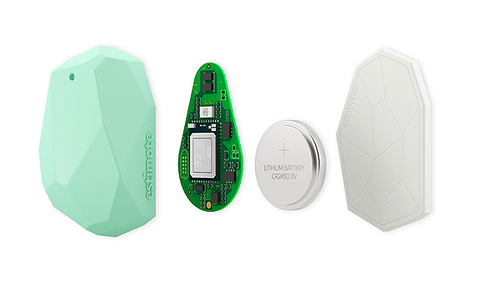
\includegraphics[width=\textwidth]{img/estimotebeacon.png}
\caption{An Estimote sticker cutaway}
\label{estimotesticker}
\end{center}
\end{figure}

With the Estimote SDK, apps on the smartphone are able to understand their proximity to nearby locations and objects, recognising their type, ownership, approximate location, temperature and motion.\\

We used these capabilities in \UB\ to develop a solution that localise a user in an indoor environment and recognise when he/she is inside or outside a specific region (the lecture's room).

\subsection{The framework}\label{estimoteframework}
The Estimote framework is build on the Core Location framework made by Apple and updated on 2014 to support the iBeacon \ref{iBeacon} technology.\\

Estimote develop this framework to wrap the Apple standard indoor functionality and extend the power of localisation by adding the support to the Estimote stickers and their functionality (such as the temperature, the signal power, the identifiers and the connection to the Estimote Cloud).\\

One of the main feature the Estimote engineers focused on is the accuracy of the indoor localisation. The frameworks provides additional support for developers that want to implement their custom localisation in the software, helping to avoid the problems that come from signals noise, peoples in the room, nearby wireless waves etc... (see \ref{indoorlocalisation}). Even if there aren't much information about \emph{how} Estimote is able to improve the quality of the localisation, it seems that they choose an higher frequency for the signal broadcast (from 1Hz specified by Apple in the iBeacon protocol to 5Hz) and a different refresh rate for their devices (less that 1s, maximum limit imposed by the iBeacon). For these reason a proprietary framework between the application and the Estimote devices is quite mandatory.

%TODO: INSERT REFERENCE HERE TO THE CHAPTER ABOUT THE TRIANGULATION PROBLEM.